\chapter{ファイル送信時におけるデータ容量と処理時間の関係について}

(時間があればもっとちゃんと書きます。)
KEKとLBLにおいてなぜ差が出るのかを考察する。
ファイル送信時におけるデータ容量と処理時間の関係は、線形性を示さない。
図\ref{datasize_vs_time_scp}はKEKからLBLのサーバーにscpコマンドを用いてファイル送信を行い、データ容量と処理時間の関係を取得したものである。
赤線が線形フィットであるが、測定点は優位にずれていることが分かる。
これはTCP通信においてパケットの送信に輻輳制御と呼ばれる技術が使われており、データ送信量を変化させながら情報通信を行っている。

\begin{figure}[bpt]\centering
  \begin{center}
    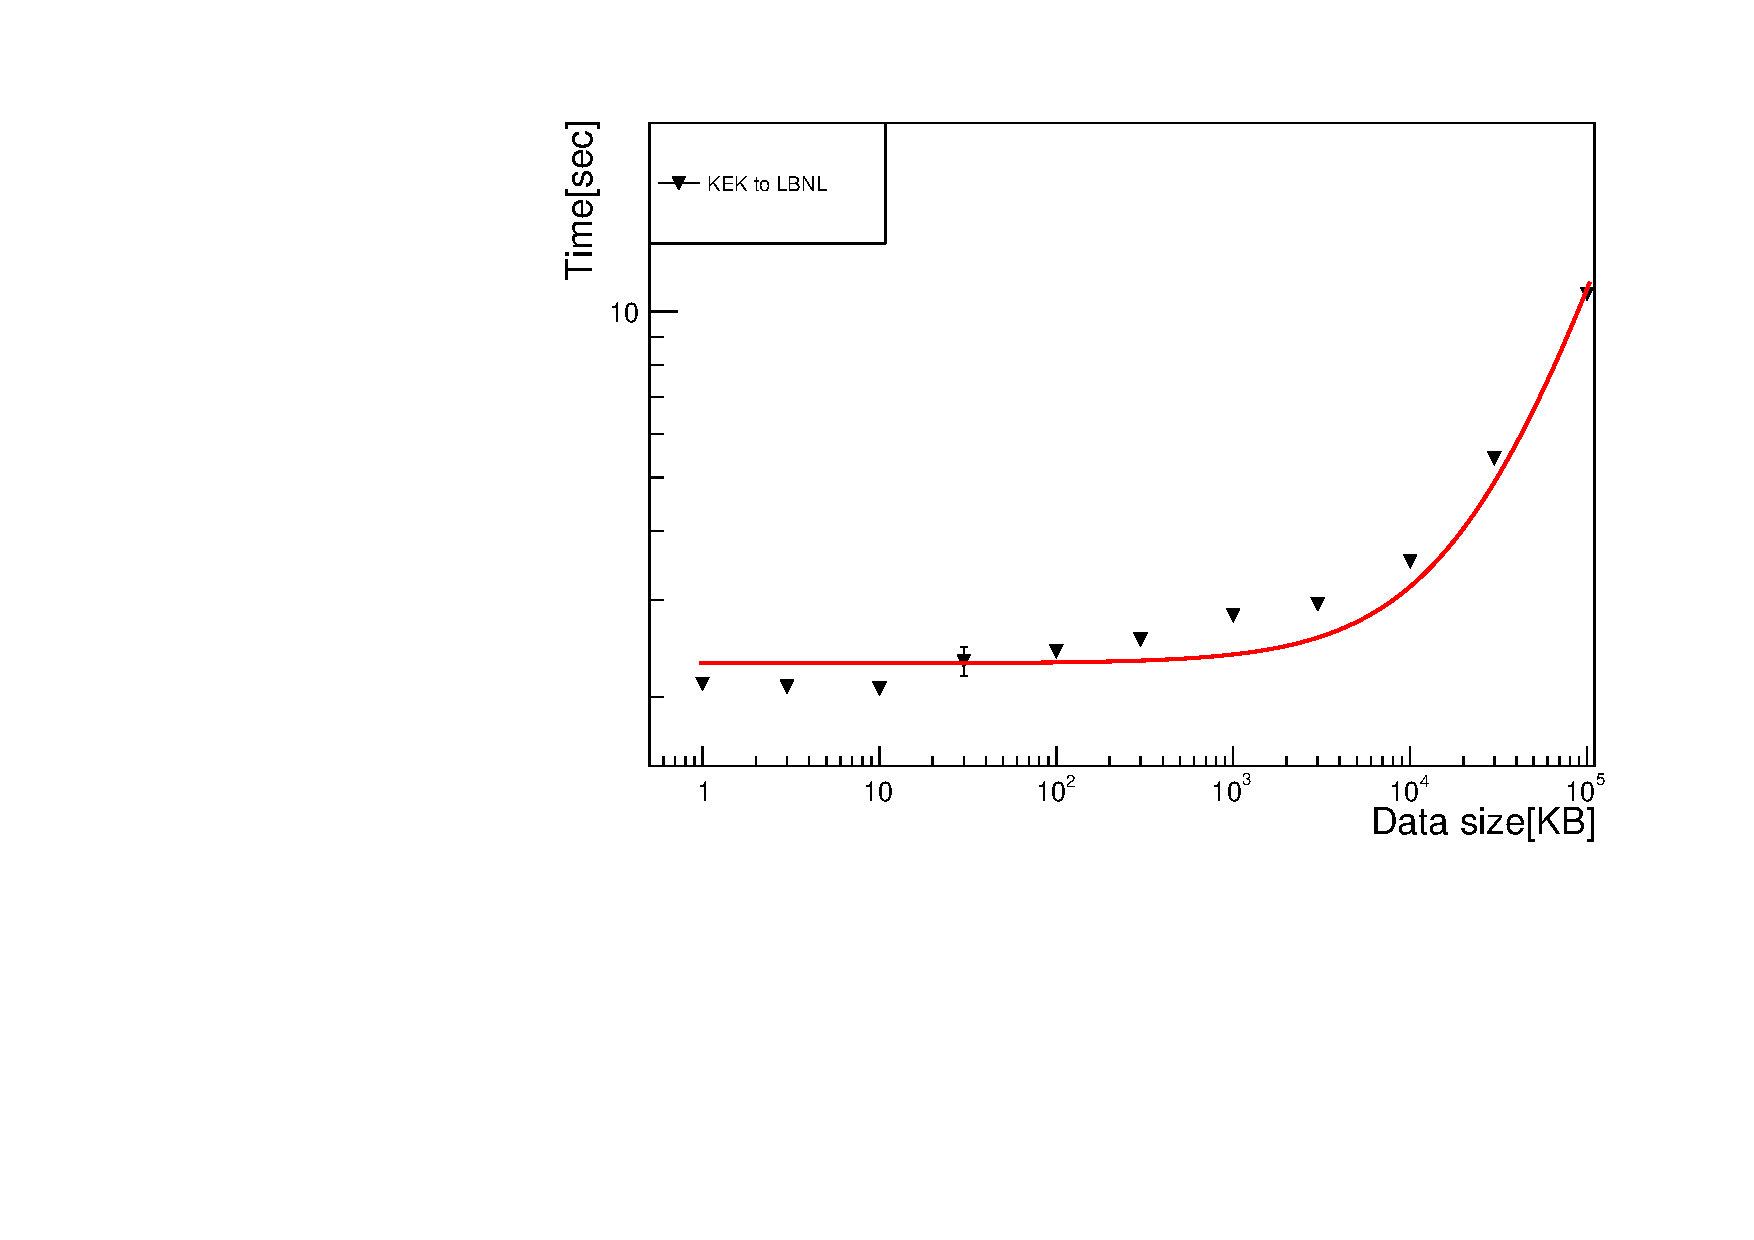
\includegraphics[width=7cm,angle=270]{datasize_vs_time_scp.pdf}
  \caption[添付するファイルサイズと処理時間の関係]{添付するファイルサイズと処理時間の関係}
  \label{datasize_vs_time_scp}
  \end{center}
\end{figure}

scpによるファイル送信をKEK->LBL、LBL->KEKの場合に対しておこなった。図\ref{datasize_vs_time_kek_lbl}のように差異が見られた。
Serverのspecは同程度。読み書き速度も変わらなかった。
輻輳制御アルゴリズム(Cubic)、Window sizeとping(111msec)は変わらなかった。
一般的には上りより下りの方が太いと考えると、KEKの上りnetworkはLBL上りと比べての方が細いと考えられる。
\begin{figure}[bpt]\centering
  \begin{center}
    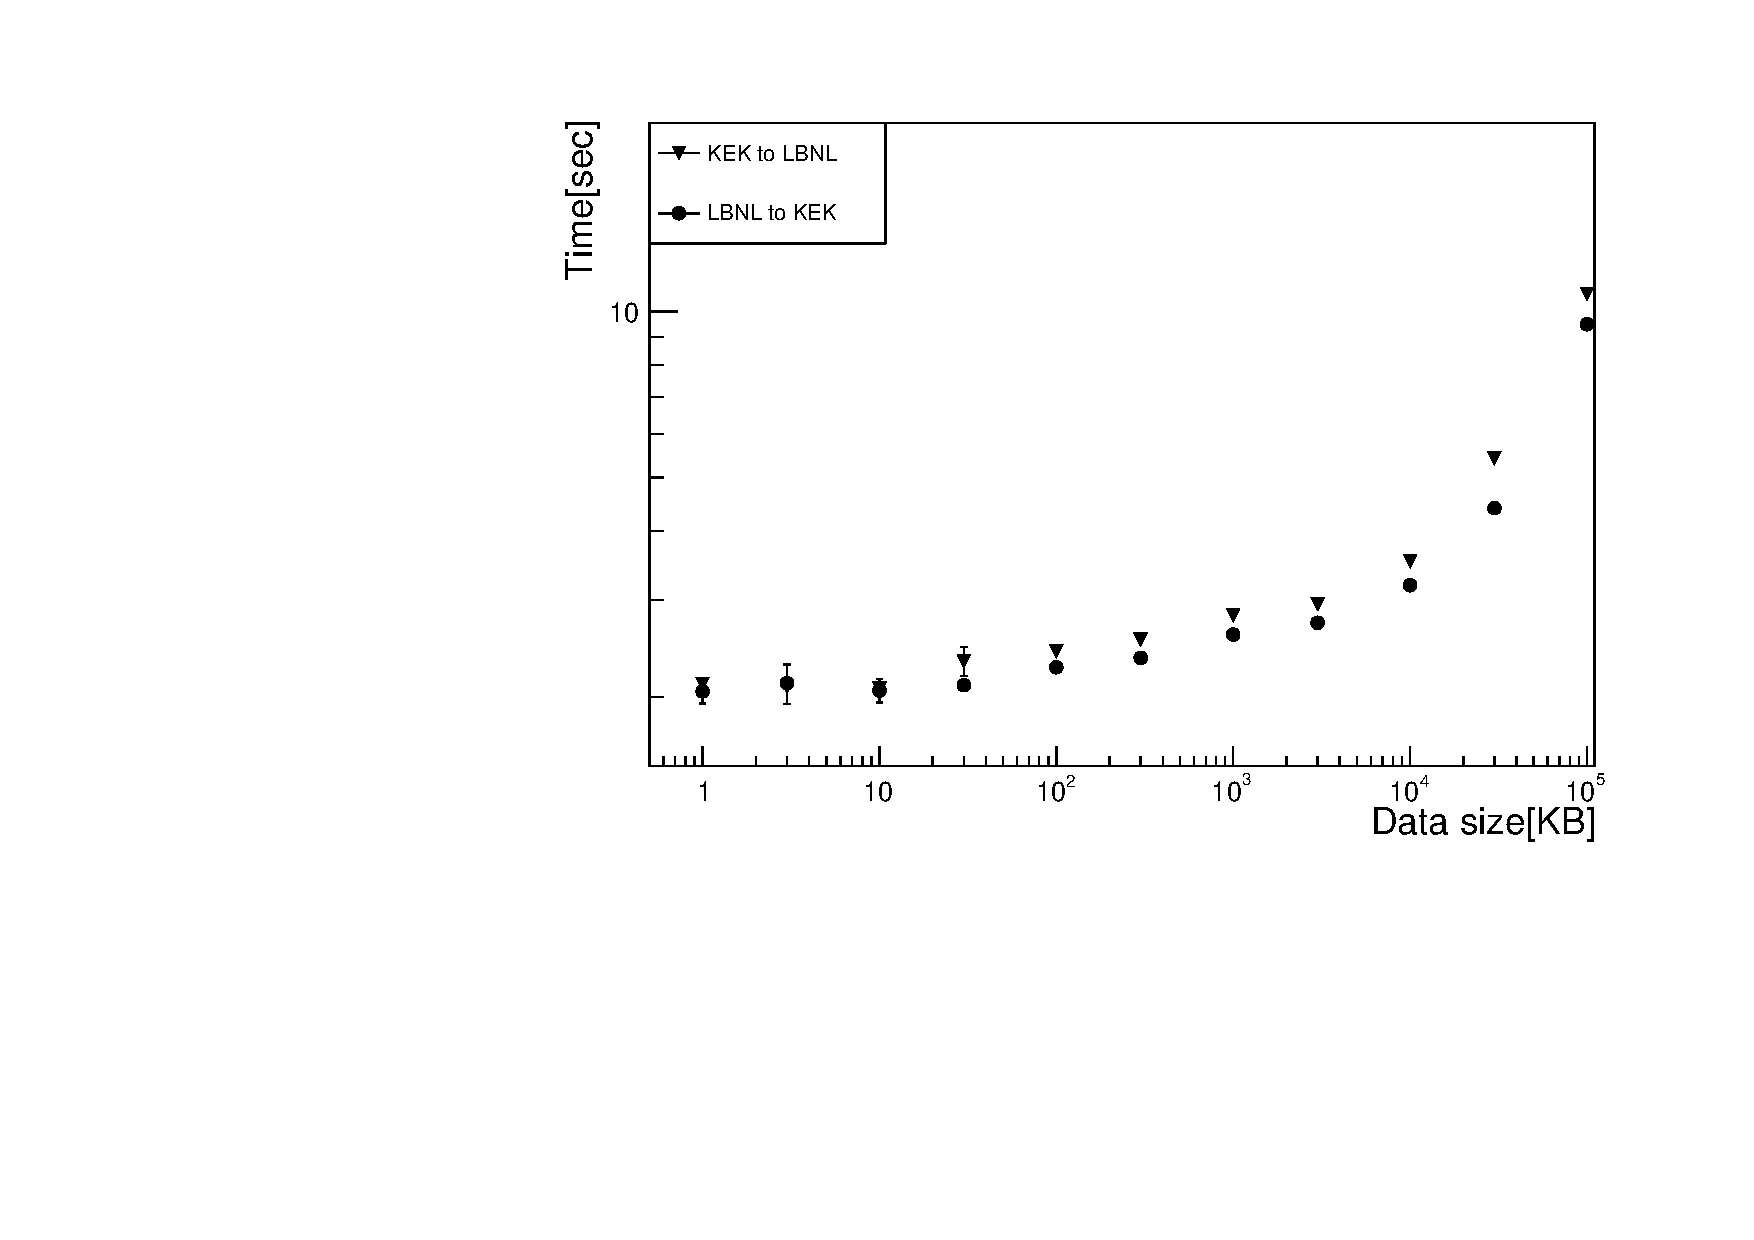
\includegraphics[width=7cm,angle=270]{scp_kek_lbl.pdf}
  \caption[KEK、LBL間のファイル送信]{KEK、LBL間のファイル送信}
  \label{datasize_vs_time_kek_lbl}
  \end{center}
\end{figure}

scpファイル送信、KEK-Lxplus、LBL->Lxplus
上述したようにKEKの上りネットワークは細い。
加えてpingによる反応時間がKEKは170msec程度なのに対し、LBLは150msec程度。ネットワーク上の距離差も処理速度影響していると考えられる。
\begin{figure}[bpt]\centering
  \begin{center}
    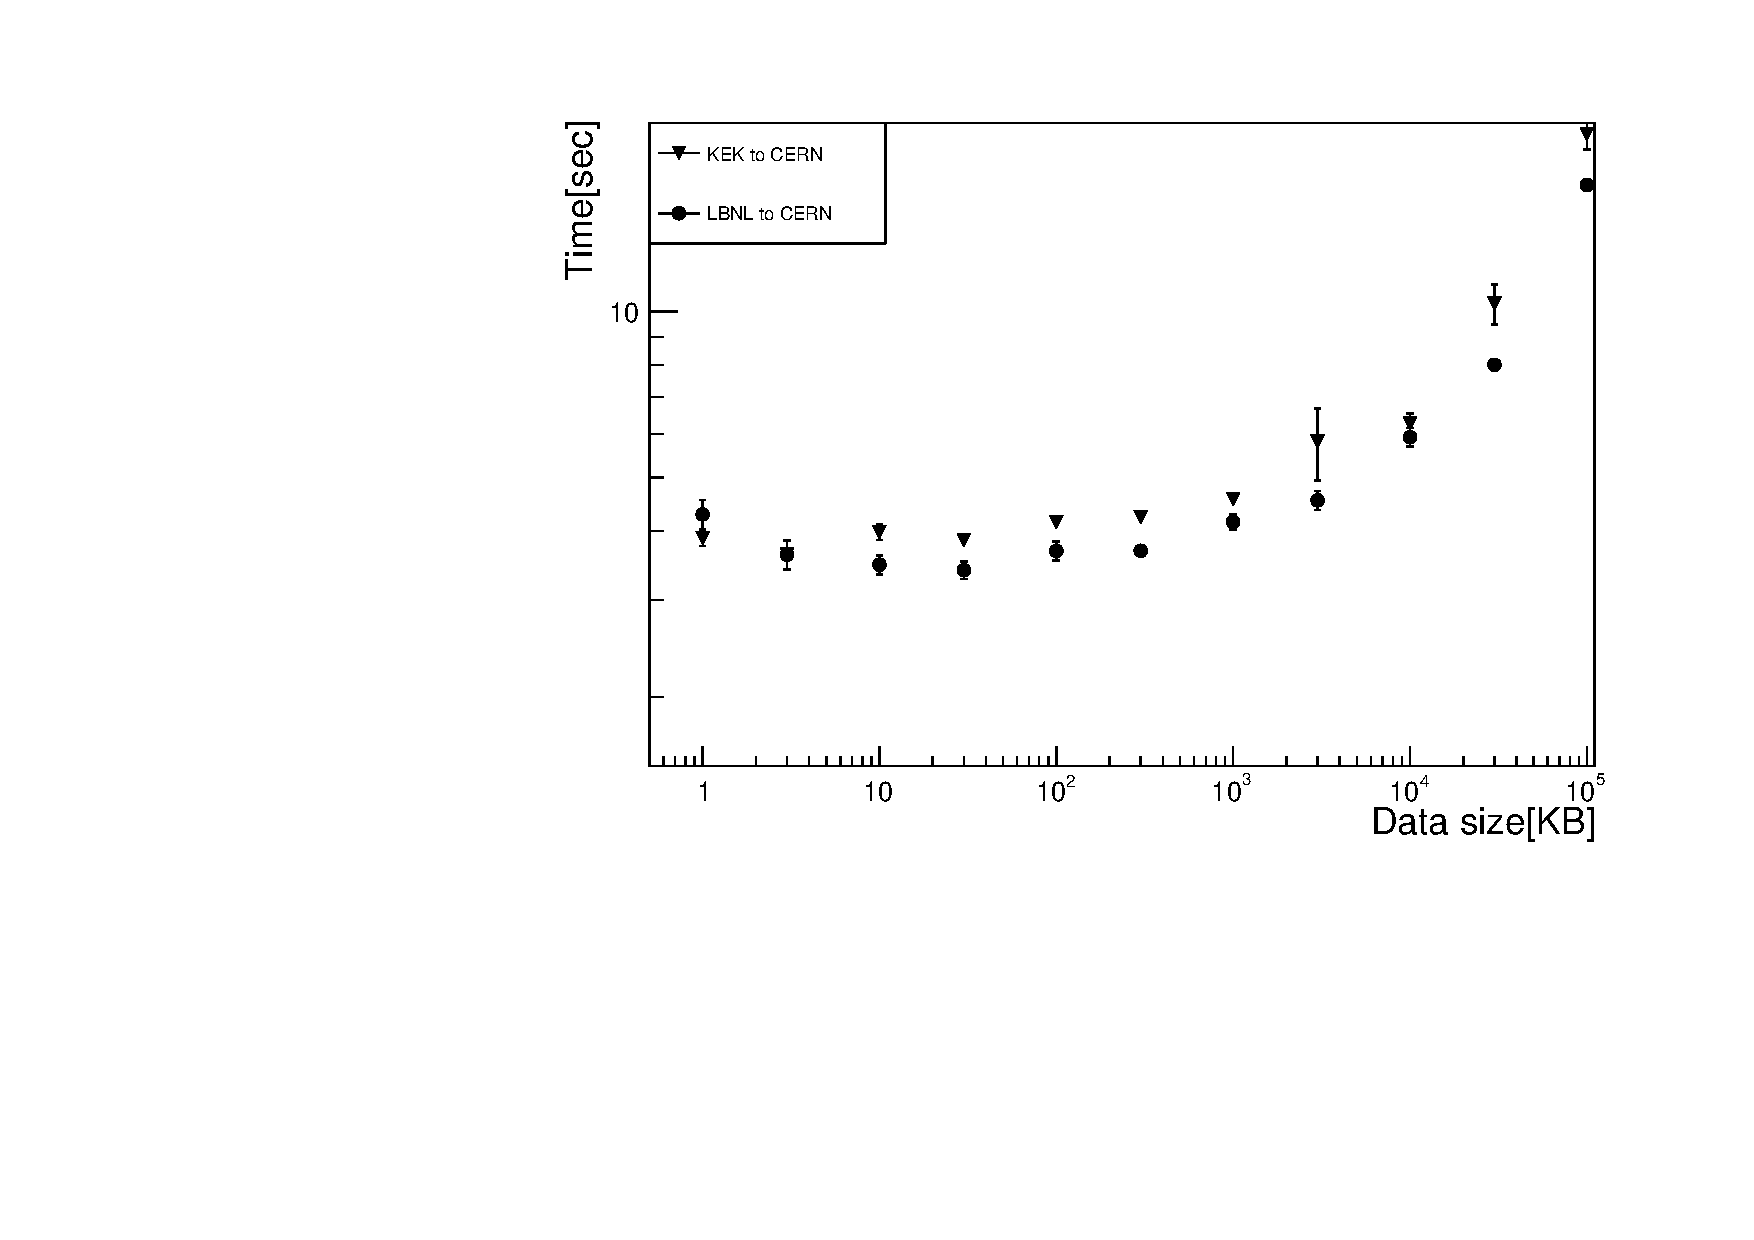
\includegraphics[width=7cm,angle=270]{scp_to_cern.pdf}
  \caption[KEK、LBLとCERN間のファイル送信]{KEK、LBLとCERN間のファイル送信}
  \label{datasize_vs_time_cern}
  \end{center}
\end{figure}

CERNと中央DBでは条件が違うが、上述したことをまとめるとKEKとLBLの間で処理時間の際が生まれる要因は以下であると考えた。
\begin{itemize}
  \item KEKの上りネットワークが遅い
  \item ネットワーク上の距離差があり、KEKの方が差が大きい。
\end{itemize}

